\section{Introduction}

\begin{figure*}[t]
 \begin{center}
  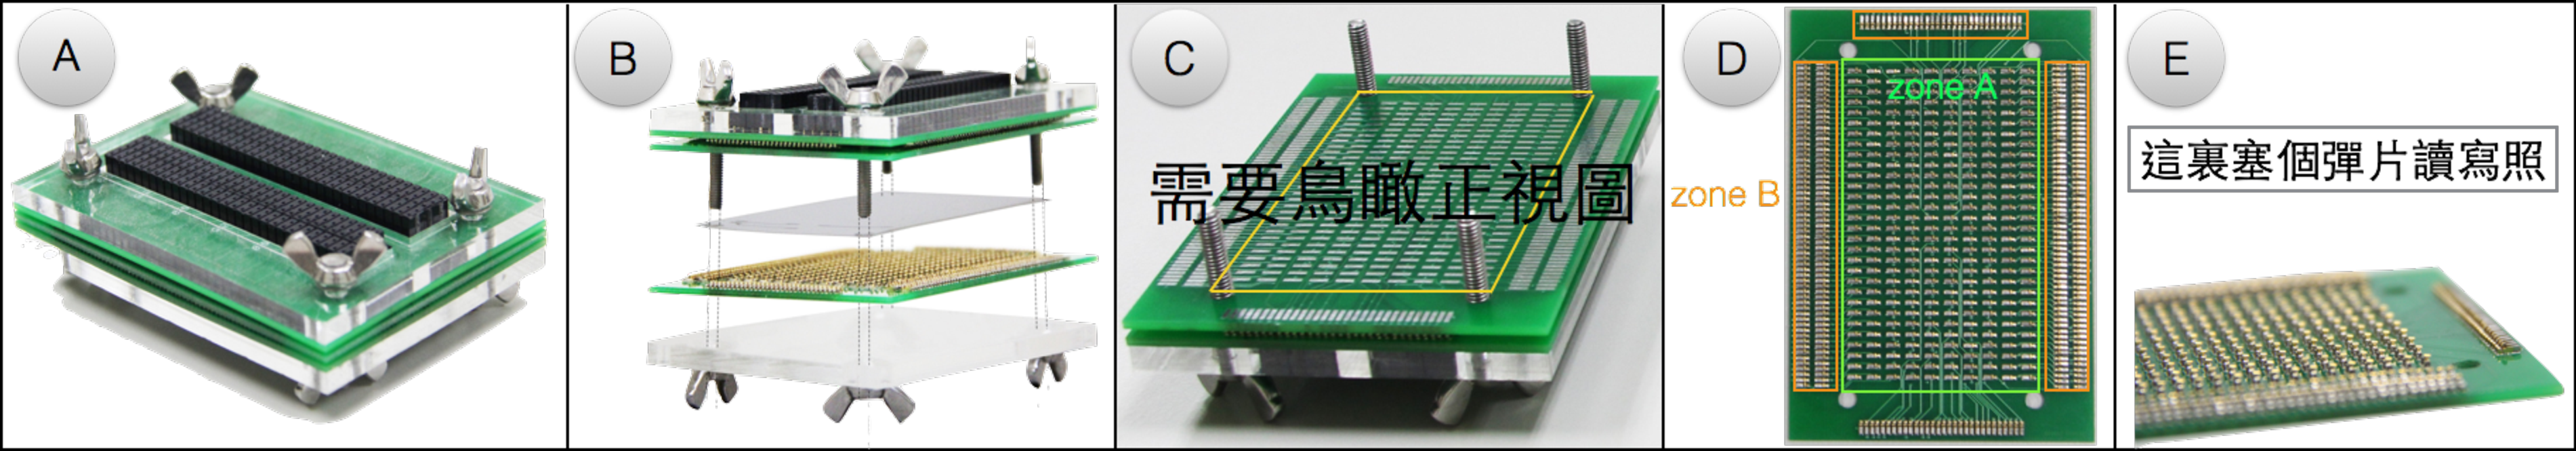
\includegraphics[width=2\columnwidth]{figures/Figure1Temp_v2.pdf}
  \caption{
    (A) 
  }
  \label{fig:System_Flow}
  \end{center}
\end{figure*}

% Breadboard is currently the dominant tool in any prototyping process. Despite its popular, breadboard is not without its flaws, namely the need for jumper cables which lead to cluttered and messy prototypes.

%Breadboard is the most popular tool for electronic circuit prototyping due to its ease of circuit modification. Though, complicated circuits involving IC chips often result in complicated wiring when using jumpers. This significantly slows down the process of prototyping because a clutter of jumper wires overlapping each other on a breadboard impairs the sight of a user leading to increased difficulty in circuit modification and placement of new components.

When it comes to electronic circuit prototyping, we often choose a breadboard due to its high modifiability. However, complicated circuits involving IC chips and jumper wires are rather muddled on breadboards. It becomes difficult for users to make changes on a breadboard when a clutter of jumper wires overlap each other, leading to the prototyping process to be significantly prolonged. %軒

%Another common tool of prototyping is the perfboard, which requires soldering jumper wires together that may take several hours to complete. A printed circuit board (PCB) allows no circuit modification, and normally takes up to 2 weeks of processing time.

Another tool known as the perfboard provides component fixation resulting in a more stable circuit, but soldering jumper wires together may take several hours to complete. A PCB normally comes up in the final stages of prototyping and takes up 1 to 2 weeks of processing time.%軒

% The recent development in electric circuit rapid prototyping tools, such as ink-based electrical circuitry allows users to prototype without wiring. Unfortunately, ink-based electrical circuitry is inherently difficult to modify, because electronic components are affixed on a piece of paper or board by soldering or taping. A hard-to-modify prototyping tool slows makers down due to component reattachment to a new printed circuitry. We therefore argue that the process of how circuit rapid prototyping is used for quick modification is not yet optimal.

% In order to allow makers to iterate quickly, hard-to-modify techniques, such as sketching and paper prototyping, give priority to speed over functionality. This trade-off pays off in the early phases of design because it encourages the quick exploration of several versions before committing further resources, eventually leading to a better design.

% We argue that the same principle should apply to circuit prototyping – a concept we call easy-to-modify circuit prototyping. In contrast to the traditional workflow, in which the circuit prototyping is always done as time-consuming soldering or hard-to-modify ink-based techniques, easy-to-modify prototyping makes all intermediate versions as fast and easy-to-modify circuits. Only at the end, when the design is finished, the complete circuit prototype is printed as PCB (Figure 2).

% One ink-based circuit prototyping approach is Inkjet — a system that prints circuits speed-up by substituting wires with conductive silver ink. Unfortunately, Inkjet requires users to attach components on the circuit with hard-to-modify approaches, such as taping or soldering.

% In this paper, we present a easy-to-modify approach that not only save time, but also save the cost of components. The key idea is to combine the mechanism of breadboard and ink-based circuit printing to provide an easy-to-modify and robust approach for circuit prototyping , i.e. a 3D print in which surfaces have been replaced with a wireframe mesh. Our approach runs on both standard FDM 3D printers, such as the PrintrBot or the Kossel mini (rather than on a 5 axis robot arm [12]) and Inkjet printers (Brothers MFC) users only need to install the uCirKit software. Resin-coated photo paper helps to maximize the conductivity of the printed wires.

% The work presented in this paper builds on rapid prototyping of circuits, the simplicity of modification on circuits, multi-layer solutions, and approaches of how to assemble components on circuits.

% \subsection{Conventional Circuit Prototyping Tools}
% A breadboard is the most popular tool for electronic circuit prototyping due to its ease of circuit modification and its ability to build all kinds of projects including simple and complicated circuits. Even though its component-pluggable mechanism requires no soldering, complicated circuits involving IC chips built on a breadboard often result in complicated wiring when using jumpers. This significantly slows down the process of prototyping because a clutter of jumper wires overlapping each other on a breadboard and blocking the sight of a user increases difficulty in circuit modification and plugging new components.

% A breadboard is the most popular tool for electronic circuit prototyping due to its ease of circuit modification. Though, complicated circuits involving IC chips built on a breadboard often result in complicated wiring when using jumpers. This significantly slows down the process of prototyping because a clutter of jumper wires overlapping each other on a breadboard that blocks the sight of a user increases difficulty in circuit modification and placement of new components.

% A perfboard is also a popular prototyping tool mainly serving a purpose for component fixation resulting in a more compact and a more stable circuit. However, building a circuit on a perfboard requires soldering and connecting jumper wires that may take several hours to complete.

% A perfboard requires soldering and connecting jumper wires that may take several hours to complete. A printed circuit board (PCB) allows no circuit modification, and it normally takes up to 2 weeks of processing time.

% A printed circuit board (PCB) is usually a final stage for prototyping that provides more freedom with respect to component positioning and a much more compact circuit. However, PCBs allow no circuit modification, and it normally takes up to 2 weeks of processing time. Thus, PCBs are currently not suitable for rapid prototyping.



% \subsection{Novel Designs in Circuit Prototyping}
% Advances in personal PCB fabrication devices and also material sciences have enabled new methods of prototyping.
% Recently, HCI researchers have proposed materials and also assembly methods for a variety of prototyping tools:
% Instant Inkjet Circuits \cite{Instant_Inkjet_Circuits} demonstrated the use of conductive ink to create printed, flexible circuits along with 3M conductive tape to provided a means of attaching components.
% Visible Breadboard \cite{Ochiai:2010:VED:1836845.1836950} presents the concept of a solder-less prototyping platform. LittleBits \cite{LittleBits} proposes an open-sourced library of modularized components as a means of prototyping.
% Circuit Stickers \cite{Circuit_Stickers} and Sketching in Circuit \cite{Sketching_in_Circuits} both utilize a form of conductive tape on paper as a tool.
% Lastly, LightUp \cite{LightUp} demonstrates an important concept in electronics, multi-layer circuits.

%Since both breadboards and perfboards require connections via jumper wires that slow down the process of prototyping and decrease the ease of use of such tools, advances in personal circuit fabrication devices and also material sciences have enabled new methods of prototyping centering on wire connections.

Aiming to solve efficiency problems in both breadboards and perfboards caused by jumper wires,
modern advances in personal circuit fabrication devices and material sciences have enabled innovative methods of prototyping centering on wire connections. Novel prototyping tools are mainly divided into three categories based on the form of the substrate for components: (1) \textit{board}, (2) \textit{conductive ink and paper electronics}, and (3) \textit{modularized electronics}.
% Recently, HCI researchers have proposed materials and also assembly methods for a variety of prototyping tools mainly divided into three categories based on the form of the substrate for the components: board, conductive ink and paper electronics, and modularized electronics.



% \subsubsection{Board}
% Previous works in the board category features a piece of hard flat substrate for electrical components.
% Visible Breadboard \cite{Visible_Breadboard} is a pluggable and jumper-wire-free prototyping platform by employing a capacitive touch layer for cable connections that averagely saves up to approximately 55\% of time compared to that of building the same circuit on a breadboard. Yet, \cite{Visible_Breadboard} is not compatible with most standardized components due to its dimensions causing inapplicability aside from elementary education.
Of the \textit{board} category, Visible Breadboard \cite{Visible_Breadboard} is a pluggable and jumper-wire-free prototyping platform that averagely saves up to approximately 55\% of time compared to that of building the same circuit on a breadboard.

% \subsubsection{Conductive Ink and Paper Electronics}
Breakthroughs in conductive ink such as Instant Inkjet Circuits \cite{Instant_Inkjet_Circuits} demonstrated the use of conductive ink to create PCP along with 3M conductive tape to provide a means of attaching components.
% \cite{Instant_Inkjet_Circuits} using off-the-shelf conventional printers and replacing the default ink with cartridges filled with silver nano-particle ink.
Although \cite{Instant_Inkjet_Circuits} claims to be a rapid prototyping tool that replaces manual wiring, PCP suffers from 2 major drawbacks. One is the single-layer issue that limits the routing of complicated circuits. Another is the poor modification ability where all components need to be reattached to a new piece of PCP after correcting a design error on a previous piece of PCP.

% Circuit Stickers \cite{Circuit_Stickers} extends the use of \cite{Instant_Inkjet_Circuits} and proposes a method to affix components using stickers to create more reliable circuits by expanding contact areas.
% Sketching in Circuit \cite{Sketching_in_Circuits} utilizes copper tape on paper as a tool to replace jumper wire connections.
% ShrinkyCircuits \cite{ShrinkyCircuits} uses a conductive pen and a heat-shrinking polymer substrate to create a solderless and jumper-wire-free circuit.
% \cite{Sketching_in_Circuits} and \cite{ShrinkyCircuits} are new forms of circuit prototyping focusing more on education, creativity, and design instead of targeting rapid prototyping for advanced hardware design and implementation.

% \cite{Circuit_Stickers}, \cite{ShrinkyCircuits}, and \cite{Sketching_in_Circuits} propose stickers for component fixation, copper tape wiring, and heat-shrinking substrate along with conductive pen, respectively, as new forms of circuit prototyping.
% However, most related work in this category focus on education, creativity, and design instead of targeting rapid prototyping for advanced hardware design and implementation.

Component fixation has been an issue in paper electronics, with the methods proposed by Circuit Stickers \cite{Circuit_Stickers}, ShrinkyCircuits \cite{ShrinkyCircuits}, and Sketching in Circuits \cite{Sketching_in_Circuits}, proper component fixation and wiring has been demonstrated.
However, most related work in this category focus on education, creativity, and design instead of targeting rapid prototyping for advanced hardware design and implementation.

% \subsubsection{Modularized Electronics}
% LittleBits \cite{LittleBits} proposes an open-sourced library of modularized components as a means of prototyping.
% LightUp \cite{LightUp} demonstrates an important concept in electronics, multi-layer circuits.

% LittleBits \cite{LittleBits} proposes modularized components which become functional by simply snapping parts together with magnets as a means of prototyping without the need of wiring and electrical expertise.
Modular circuit construction such as LittleBits \cite{LittleBits} proposes modularized components using a magnetic-snapping mechanism as a mean of prototyping without the need of wiring and electrical expertise.
% LightUp \cite{LightUp} transforms electrical components into blocks assisting beginners to explore fundamental concepts of engineering and electronics.
LightUp \cite{LightUp} transforms electrical components into blocks assisting beginners to learn electronics.
Despite \cite{LittleBits} and \cite{LightUp} being rapid prototyping tools, the encapsulation of hardware details leads to impracticability under scenarios requiring customized components and complicated circuits.

Among the related works, a breadboard provides easy modification by its pluggable mechanism, and PCP offers fast wiring by printing out conductive ink. Thus, we implemented a new rapid prototyping tool with a multilayer design, \papertitle, simultaneously adopting a pluggable mechanism via female headers on the top layer and PCP fast wiring mechanism on the bottom layers. 
% \papertitle\ is a multilayer design where the top layer is the component-pluggable mechanism implemented by female headers and PCP is placed in the bottom layers to arrange connections.

Whether the combination of the benefits results in faster prototyping times is of interest. Hence, both a breadboard and PCP should be evaluated as a basis of comparison to \papertitle. However, \cite{Circuit_Stickers} suggests that the 3M conductive tape has poor reliability in component connection. To verify this, we imitate Figure 7b in \cite{Instant_Inkjet_Circuits} and conclude that only 18\% of the pins are electrically connected to the conductive ink through the 3M tape. Thus, we remove PCP from our evaluation.

Our user study shows that our system is slightly inefficient under simple circuits but becomes powerful when building complicated ones. In terms of overall work time, \papertitle\ has a significant improvement in overall prototyping performance by 43\% and a considerable decrease in debug time by 78\% compared with that of a breadboard.

% \subsection{Circuit Printing Technology}
% The core of our work is circuit printing technology. In the work Instant Inkjet Circuits, the authors proposed a method in which they used off-the-shelf conventional printers and replaced the default ink with cartridges filled with silver nano-particle ink. This opens up circuit printing technology for the masses. Not only does such a work deliver rapid circuit creation, but also opens up a possibility of rapid prototyping, which we will discuss more in the next subsection.

% \subsection{Rapid Prototyping}
% Currently, a big player in the prototyping world is LittleBits. LittleBits seeks to modularize components and reduce the difficulty of prototyping with sophisticated electronics an elementary task. Such a feat is achieved by utilizing materials such as cardboard and paper and creating tiny circuit boards out of these materials. Along with the tiny circuits, magnets provide a mechanism for attaching differing components together to prototype complicated circuits. But besides LittleBits, Visible Breadboard presents a breadboard-like routing board that employs a capacitive touch layer for cable connections. An intuitive method such as capacitive touch showed immense improvement over soldering solutions. The last member of popular prototyping methods is the application of conductive tape as a means of connection, as well as fixing components in place. Both Circuit Stickers and Sketching in Circuit are proponents of this method.

% \subsection{Multi-layer Prototyping}
% Despite the various kinds of rapid prototyping tools, multi-layer circuits are a difficult task for current methods. LightUp utilizes a stacking method in which electronic components can be layered on top of each other to create multi-layer prototyping. This third dimension allows for a third direction in which circuits can expand, and also simplifies design of complicated circuits.